%%%%%%%%%%%%%%%%%%%%%%%%%%%%%%%%%%%%%%%%%%%%%%%%%%%%%%%%%%%%%%%%%%%%%%%%%%%%%%%%
% Thesis / Project Report
% LaTeX Template
% Version 2.0 (08/04/16)
%
% Author:
% Siddhant Shrivastava
% https://github.com/sidcode/bits-pilani-thesis-template-latex
%
% This template is heavily based on the work of Darshit Shah, Steven Gunn and Sunil Patel
% Darshit Shah
% https://github.com/darnir/BPHC-LaTeX-Report-Class
% Steven Gunn
% http://users.ecs.soton.ac.uk/srg/softwaretools/document/templates/
% and
% Sunil Patel
% http://www.sunilpatel.co.uk/thesis-template/
%
% License:
% CC BY-NC-SA 4.0 (http://creativecommons.org/licenses/by-nc-sa/4.0/)
%
% Note:
% Make sure to edit document variables in the Thesis.cls file
%
%%%%%%%%%%%%%%%%%%%%%%%%%%%%%%%%%%%%%%%%%%%%%%%%%%%%%%%%%%%%%%%%%%%%%%%%%%%%%%%%

%-------------------------------------------------------------------------------
%	PACKAGES AND OTHER DOCUMENT CONFIGURATIONS
%-------------------------------------------------------------------------------

\documentclass[11pt, a4paper, oneside]{Thesis} % Paper size, default font size
                                               % and one-sided paper

\graphicspath{{Pictures/}} % Specifies the directory where pictures are stored

\usepackage[backend=biber]{biblatex}

\usepackage{mathrsfs}

\usepackage{physics}

\usepackage{amsmath}

\bibliography{Bibliography.bib}

\title{\ttitle} % Defines the thesis title - don't touch this

\begin{document}

\frontmatter % Use roman numbering style (i, ii...) for the pre-content pages

\setstretch{1.3} % Line spacing of 1.3

% Define page headers using FancyHdr package and set up for one-sided printing
\fancyhead{} % Clears all page headers and footers
\rhead{\thepage} % Sets the right side header to show the page number
\lhead{} % Clears the left side page header

\pagestyle{fancy} % Finally, use the "fancy" page style to implement the
                  %FancyHdr headers

% Input all the variables used in the document. Please fill out the
% variables.tex file with all your details.
%-------------------------------------------------------------------------------
%	DOCUMENT VARIABLES
%
%	Fill in the lines below to set the various variables for the document
%-------------------------------------------------------------------------------

%-------------------------------------------------------------------------------
% Your thesis title - this is used in the title and abstract
% Command: \ttitle
\thesistitle{Determining the Mobility of Charge Carriers in Organic Semiconductors}
%-------------------------------------------------------------------------------
% The document type: Thesis / report, etc.
% Command: \doctype
\documenttype{Masters' Thesis}
%-------------------------------------------------------------------------------
% Your supervisor's name - this is used in the title page
% Command: \supname
\supervisor{Dr. Jarvist M \textsc{Frost}}
%-------------------------------------------------------------------------------
% The supervisor's position - Used on Certificate
% Command: \suppos
\supervisorposition{}
%-------------------------------------------------------------------------------
% Supervisor's institute
% Command: \supinst
\supervisorinstitute{Imperial College, London}
%-------------------------------------------------------------------------------
% Your Co-Supervisor's name
% Command: \cosupname
\cosupervisor{Dr. Pritam K \textsc{Jana}}
%-------------------------------------------------------------------------------
% Co-Supervisor's Position - Used on Certificate
% Command: \cosuppos
\cosupervisorposition{Asst. Professor}
%-------------------------------------------------------------------------------
% Co-Supervisor's Institute
% Command: \cosupinst
\cosupervisorinstitute{BITS-Pilani Pilani Campus}
%-------------------------------------------------------------------------------
% Your Examiner's name. Not currently used anywhere.
% Command: \examname
\examiner{}
%-------------------------------------------------------------------------------
% Name of your degree
% Command: \degreename
\degree{Master of Science}
%-------------------------------------------------------------------------------
% The BITS Course Code for which this report is written
% COmmand: \ccode
\coursecode{BITS F421T}
%-------------------------------------------------------------------------------
% The name of the Course
% Command: \cname
\coursename{Thesis}
%-------------------------------------------------------------------------------
% Your name. Extend manually in case of multiple authors
% Command: \authornames
\authors{Pranay \textsc{Venkatesh}}
%-------------------------------------------------------------------------------
% Your ID Number - used on the Title page and abstract
% Command: \idnum
\IDNumber{2019B2A11004P}
%-------------------------------------------------------------------------------
% Your address
% Command: \addressnames
\addresses{}
%-------------------------------------------------------------------------------
% Your subject area
% Command: \subjectname
\subject{Chemistry}
%-------------------------------------------------------------------------------
% Keywords for this report.
% Command: \keywordnames
\keywords{Polarons, Path Integrals, Quantum Dynamics, Photovoltaics, Organic Semiconductors, Mobility}
%-------------------------------------------------------------------------------
% University details
% Command: \univname
\university{\texorpdfstring{\href{http://www.bits-pilani.ac.in/} % URL
                {Birla Institute of Technology and Science Pilani}} % University name
                {Birla Institute of Technology and Science Pilani}}
%-------------------------------------------------------------------------------
% University details, in Capitals
% Command: \UNIVNAME
\UNIVERSITY{\texorpdfstring{\href{http://www.bits-pilani.ac.in/} % URL
                {BIRLA INSTITUTE OF TECHNOLOGY AND SCIENCE PILANI}} % name in capitals
                {BIRLA INSTITUTE OF TECHNOLOGY AND SCIENCE PILANI}}

%-------------------------------------------------------------------------------
% Campus Name
% Command: \campusname
\campus{Pilani Campus}

%-------------------------------------------------------------------------------
% Campus Name, in capitals
% Command: \CAMPUSNAME
\CAMPUS{PILANI CAMPUS}


%-------------------------------------------------------------------------------
% Department Details
% Command: \deptname
\department{\texorpdfstring{\href{http://www.bits-pilani.ac.in/pilani/} % Your department's URL
                {Chemistry}} % Your department's name
                {Chemistry}}
%-------------------------------------------------------------------------------
% Department details, in Capitals
% Command: \DEPTNAME
\DEPARTMENT{\texorpdfstring{\href{http://www.bits-pilani.ac.in/pilani/computerscience/ComputerScience} % Your department's URL
                {COMPUTER SCIENCE \& INFORMATION SYSTEMS}} % Your department's name in capitals
                {COMPUTER SCIENCE \& INFORMATION SYSTEMS}}
%-------------------------------------------------------------------------------
% Research Group Details
% Command: \groupname
\group{\texorpdfstring{\href{Research Group Web Site URL Here (include http://)}
                {Research Group Name}} % Your research group's name
                {Research Group Name}}
%-------------------------------------------------------------------------------
% Research Group Details, in Capitals
% Command: \GROUPNAME
\GROUP{\texorpdfstring{\href{Research Group Web Site URL Here (include http://)}
                {RESEARCH GROUP NAME (IN BLOCK CAPITALS)}}
                {RESEARCH GROUP NAME (IN BLOCK CAPITALS)}}
%-------------------------------------------------------------------------------
% Faculty details
% Command: \facname
\faculty{\texorpdfstring{\href{Faculty Web Site URL Here (include http://)}
                {Faculty Name}}
                {Faculty Name}}
%-------------------------------------------------------------------------------
% Faculty details, in Capitals
% Command: \FACNAME
\FACULTY{\texorpdfstring{\href{Faculty Web Site URL Here (include http://)}
                {FACULTY NAME (IN BLOCK CAPITALS)}}
                {FACULTY NAME (IN BLOCK CAPITALS)}}
%-------------------------------------------------------------------------------


%-------------------------------------------------------------------------------
%   NON-CONTENT PAGES
%-------------------------------------------------------------------------------
\maketitle
\Declaration
\Certificate
\Quotation{Insert Random Quote here. Publish like a boss.}{Your Name}

\begin{abstract}
The Thesis Abstract is written here (and usually kept to just this page).
The page is kept centered vertically so can expand into the blank space above
the title too\ldots
\end{abstract}

\begin{acknowledgements}
The acknowledgements and the people to thank go here, don't forget to include
your project advisor\ldots
\end{acknowledgements}

%-------------------------------------------------------------------------------
%	LIST OF CONTENTS/FIGURES/TABLES PAGES
%-------------------------------------------------------------------------------

% The page style headers have been "empty" all this time, now use the "fancy"
% headers as defined before to bring them back
\pagestyle{fancy}

\lhead{\emph{Contents}} % Set the left side page header to "Contents"
\tableofcontents % Write out the Table of Contents

% Set the left side page header to "List of Figures"
\lhead{\emph{List of Figures}}
\listoffigures % Write out the List of Figures

 % Set the left side page header to "List of Tables"
\lhead{\emph{List of Tables}}
\listoftables % Write out the List of Tables

%-------------------------------------------------------------------------------
%	ABBREVIATIONS
%-------------------------------------------------------------------------------

\clearpage % Start a new page

 % Set the line spacing to 1.5, this makes the following tables easier to read
\setstretch{1.5}

\lhead{\emph{Abbreviations}} % Set the left side page header to "Abbreviations"
\listofsymbols{ll} % Include a list of Abbreviations (a table of two columns)
{
\textbf{LAH} & \textbf{L}ist \textbf{A}bbreviations \textbf{H}ere \\
%\textbf{Acronym} & \textbf{W}hat (it) \textbf{S}tands \textbf{F}or \\
}

%-------------------------------------------------------------------------------
%	PHYSICAL CONSTANTS/OTHER DEFINITIONS
%-------------------------------------------------------------------------------

\clearpage % Start a new page

% Set the left side page header to "Physical Constants"
\lhead{\emph{Physical Constants}}

 % Include a list of Physical Constants (a four column table)
\listofconstants{lrcl}
{
Speed of Light & $c$ & $=$ & $2.997\ 924\ 58\times10^{8}\ \mbox{ms}^{-\mbox{s}}$ (exact)\\
% Constant Name & Symbol & = & Constant Value (with units) \\
}

%-------------------------------------------------------------------------------
%	SYMBOLS
%-------------------------------------------------------------------------------

\clearpage % Start a new page

\lhead{\emph{Glossary}} % Set the left side page header to "Symbols"

\listofnomenclature % List the nomenclature. (We use the glossaries package)

%-------------------------------------------------------------------------------
%	DEDICATION
%-------------------------------------------------------------------------------

\setstretch{1.3} % Return the line spacing back to 1.3

\pagestyle{empty} % Page style needs to be empty for this page

% Dedication text
\Dedicatory{Dedicate this to someone, anyone.}

\addtocontents{toc}{\vspace{2em}} % Add a gap in the Contents, for aesthetics

%-------------------------------------------------------------------------------
%	THESIS CONTENT - CHAPTERS
%-------------------------------------------------------------------------------

\mainmatter % Begin numeric (1,2,3...) page numbering

\pagestyle{fancy} % Return the page headers back to the "fancy" style

% Include the chapters of the thesis as separate files from the Chapters folder
% Uncomment the lines as you write the chapters

% Chapter Template

\chapter{Introduction} % Main chapter title

\label{Chapter1} % Change X to a consecutive number; for referencing this chapter elsewhere, use \ref{ChapterX}

\lhead{Chapter 1. \emph{Introduction}} % Change X to a consecutive number; this is for the header on each page - perhaps a shortened title

\section{Semiconductor Materials}

%What are semiconductors and why are they cool

For a variety of reasons, scientists have taken a great deal of interest in understanding how electrons behave in solids. We can figure out a few structural properties of materials from simply looking at a solid's crystal structure, but if we're interested in harnessing all of the material potential a solid can offer, we need to dive deep into what the electrons are doing. In the early 19th century, some scientists started to take notice of the fact that certain materials were conductive under very specific conditions and in 1874, Karl Braun discovered a junction contact between metal sulphides and pointed metal tips that has the  ability to rectify AC to DC current \cite{lukasiak2010history}. Unwittingly, he had discovered the metal-semiconductor junction!

In the 1930s, after the development of quantum mechanics and quantum statistics, scientists started coming up with better models of solids and started to understand the electrical conductivity of different materials in terms of their band structure.

% Band structure bit more explanation + diagram of MOs forming bands in solids. 

Based on the band structure, scientists were then able to classify materials as conductors, semimetals, semiconductors and insulators.

In 1947, Bardeen, Brittain and Shockley at Bell Labs invented the transistor, a tiny device that could switch electrical signals on and off, or amplify them. This was a breakthrough that lead the foundation for analog and digital electronics. In 1958, Jack Kilby at Texas Instruments unveiled the Integrated Circuit (IC), which was composed of several transistors, resistors and capacitors all combined on a single substrate, paving the way for the modern computing era.

% Re-write the photovoltaics para a bit.

In the 1950s and 1960s, researchers began experimenting with semiconductor materials for converting sunlight into electricity, leading to the development of solar cells. The first practical photovoltaic (PV) cells were made of silicon, a semiconductor material. Over the years, advancements in semiconductor technology, such as the development of multi-junction solar cells and thin-film technologies, have significantly improved the efficiency and affordability of solar panels.In the 1950s and 1960s, researchers began experimenting with semiconductor materials for converting sunlight into electricity, leading to the development of solar cells. The first practical photovoltaic (PV) cells were made of silicon, a semiconductor material. Over the years, advancements in semiconductor technology, such as the development of multi-junction solar cells and thin-film technologies, have significantly improved the efficiency and affordability of solar panels.


% How scientists started using different materials over time for various applications, from Si -> GaAs -> GaN -> Organics.


% For organics, talk about OLEDs a bit (rewrite the OLED para)

Semiconductor materials have also revolutionized the display industry. Liquid Crystal Displays (LCDs), introduced in the 1960s, utilize the properties of liquid crystals, which are organic semiconductor materials. The development of Organic Light-Emitting Diodes (OLEDs) in the 1980s marked another milestone. OLEDs consist of organic semiconductor compounds that emit light when an electric current is applied. OLED displays offer vibrant colors, high contrast ratios, and flexibility, making them ideal for various applications, including smartphones, TVs, and wearable devices.


% Try summarising https://www.feynmanlectures.caltech.edu/III_14.html in its entirety generally.

%Bloch's theorem somewhere here


%Electrons in a solid, Kronnig-Penny for demonstrating bands

A simple quantum mechanical model of an electron in a 1D lattice is the Kronig-Penney model, where the periodic potential of lattice atom sites is approximated by a square well potential.

% diagram of KP potential and actual atomic sites potential.

As per the Kronig-Penney model, periodically after distances of $a$ where the potential is 0, we get a constant large potential $V_0$ for an interval $b$.

We can obtain a solution for the momentum states $k$ \cite{ashcroft2022solid}, which is the following implicit equation:

\begin{equation}
\cos(ka) = \cosh(\alpha a) + P \frac{\sinh(\alpha a)}{\alpha a}
\end{equation}

Where $\alpha = (\frac{2mE}{\hbar^2})^{1/2}$ and $P = \frac{mV_0 ba}{\hbar^2}$.

To get the dispersion relation E vs k, we can vary E and get the right-hand side of the above relation, from which we can take $\arccos$ on both sides of the equation to get k. 

% Plot of RHS vs alpha/a

Naturally, when the right hand side of the equation is outside of $[-1, 1]$, the inverse cosine does not exist and certainly this is what happens for quite a range of E values and is the reason we see, among other things, a band-gap obtained in the resulting dispersion relation.

% E-k diagram in Kronig-Penney.





%Mobility, Einstein-Smoluchowski Relation.

%simple p-n junction because why not.

%Photovoltaics and their importance in modern context of energy materials

%Shockley Queisser limit with proof. Mention multijunction as one way of overcoming but processes in organic materials more interesting.

%Organic photovoltaics are taking off.



\section{Electronic Structure}

The electronic structure is the solution of the quantum states of electrons in a given chemical system. Typically, this involves determining the energies and wavefunctions of the various states. This can be done by solving the Schr{\"o}dinger equation for molecules.


\subsection{Tight-binding Model of Solids}

\subsection{Density Functional Theory}

% DFT, TD-DFT, DFTB

\subsection {Complete Active Space Methods}

When studying electronic structure, the first accurate method proposed was the Hartree-Fock (HF), where we reduce the electronic Hamiltonian into effective one-electron operators using a mean-field description :

\begin{equation}
    \mathcal{H}_e = \sum_{i} f(i) = \sum_{i}[ -\frac{1}{2} \nabla_i^2 - \sum_A \frac{Z_A}{r_{iA}} + \nu^{HF}(i)]
\end{equation}

Where $\nu(i)$ represents the electron-electron interactions in an averaged-out fashion. The post-Hartree Fock methods were devised to tackle the challenge of dynamical correlation that's left out in the mean-field approach described in the HF method. One way of doing this is to construct a wavefunction that uses a linear combination of Slater Determinants : 

\begin{equation}
\ket{\psi} = c_0 \ket{\psi_0} + c_1 \ket{\psi_1} + c_2 \ket{\psi_2} + ...
\end{equation}

Where $\ket{\psi_0}$ is the Hartree Fock ground state determinant. The most accurate wavefunction electronic structure theory method that has been developed is the Full Configurational Interaction or Full-CI method, which uses all possible excited determinants in the linear combination. For a given basis set of K functions, it is the most accurate method, however the number of determinants to include in the expansion is extraordinarily large: $2K \choose N$ for an N electron system. One way to reduce computational costs is to study a small number of excitations, say just single or double excitations, leading to a truncation in the wavefunction expression. These are called truncated CI methods, for example CIS and CISD which only use single and double excitations respectively. Another approach is to also use the Multiconfigurational Self-Consistent Field method, where we construct a truncated CI wavefunction $\ket{\psi} = \sum_I c_I \ket{\psi_I (\{a_i\})}$ but instead of varying just the coefficients $c_I$ we also vary the coefficients $\{a_i\}$, leading to a non-linear variational problem. However, due to the size-consistency problem, truncated CI methods do not scale very well for many-electron systems \cite{szabo2012modern}.

For many problems in chemistry, we are only interested in a small number of excited state properties. We can hence select an "Active Space" of orbitals which contains the properties of excitations we're interested in, typically some valence orbitals and few virtual orbitals. 

% Complete Active Space diagram.

Within this active space, we can consider all possible excitations and since we're only choosing a small number of orbitals to work with, the number of excitations is not too large to perform our calculations. We can perform MCSCF calculations within this Active Space using all excitations, this is known as the Complete Active Space Self Consistent Field (CASSCF). Instead, if we perform a full CI calculation within the complete active space, it's called Complete Active Space Configuration Interaction or CASCI. We can also use the CASSCF result as a reference for performing 2nd or 4th order  M{\o}ller-Plesset perturbation theory calculations, which are the CASPT2 methods. 

One method that leverages the active space idea but reduces computational cost is the family of Reduced Active Space RASSCF methods. Instead of treating the entire space completely, we can divide the space into three parts, where we treat one part completely and consider only some excitations into and out of this part.

% RASSCF diagram.


When attempting to study exciting processes in organic photovoltaic materials such as multi-exciton generation, methods such as CIS and TD-DFT fail to capture these effects and that's where we find the CASSCF and related methods particularly helpful \cite{zimmerman2013correlated}.




\section{Phonons}

% What are phonons

% Sample phonon dispersion in a solid.

% How to get phonons from electronic structure calculations in solids (phonopy or something of that order).

% Why treating el-ph interactions in solids is important.




% Chapter Template

\chapter{Organic Semiconductors} % Main chapter title

\label{Chapter2} % Change X to a consecutive number; for referencing this chapter elsewhere, use \ref{ChapterX}

\lhead{Chapter 2. \emph{Organic Semiconductors}} % Change X to a consecutive number; this is for the header on each page - perhaps a shortened titl

\section{Introduction}

Organic molecular solids have attracted attention for a variety of applications, as structural materials, in medicine and as semiconductors, for classical transistor applications as OFETs (Organic Field Effect Transistors), or in optoelectronics as OLED (Organic Light Emitting Diode) display materials and OPV (Organic Photovoltaics) solar cells.

One of the issues with photovoltaic materials is the Shockley-Queisser limit, which is a theoretical limit for the efficiency of a solar cell. We exploit interesting properties of organic materials to overcome this limit to get highly efficient solar cells, specifically singlet fission and upconversion. Materials such as Y6 have showcased impressive efficiencies near 20\%  [cite].

\section{Excited States}

In organic materials, we are interested in two types of excited states : singlets and triplets. 

Excited singlet states are formed when an electron gets excited such that the overall spin quantum number s = 0 (the multiplicity hence being 2s + 1 = 1)

% Diagram for singlet state in a dimer. 

Excited triplet states are formed when an electron gets excited such that the overall spin quantum number s = 1 (the multiplicity hence being 2s + 1 = 3). 

% Diagram for triplet state in a dimer.

For the example a dimer, the excited state can also form a charge transfer (CT) state.



\section{Singlet Fission}

% Try writing the entirety of Smith-Michl 2010, 2013 and Casanova 2018 here in your own words. This should bulk up the document by a significant amount.


Singlet fission is a photophysical process that may allow us to improve photoconversion efficiencies in solar cells. This is a downconversion photophysical process where an excited singlet state evolves into two spin-triplets, often observed in organic materials \cite{casanova2018theoretical} \cite{smith2010singlet}.

\begin{equation}
    S^{*} \to T_1 + T_1
\end{equation}

\begin{figure}
\centering
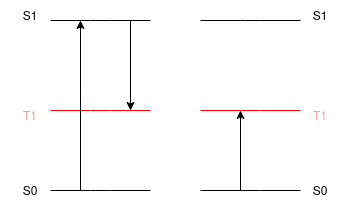
\includegraphics[scale=0.6]{Figures/SF.png}
\caption{Singlet Fission process in a dimer of chromophores}
\end{figure}

As is the case in other internal conversion processes in organic materials it can be very fast, happening at a sub-$ps$ time scale. Despite a large amount of research being devoted to research in singlet fission in organic materials we do not fully understand the mechanisms that underlie this process. 

Singlet fission was first observed by Singh and Stoicheff in 1963 [cite] when they identified intermediate states in anthracene that were able to absorb two photons. Subsequently in the 1960s and 70s, several articles were published around understanding the decay of singlet states into a pair of triplet states and the reverse process, where triplet states annihilate to generate singlets. Kinetic models were developed to try to model singlet fission but were not very successful at reproducing the experimental findings. Since then, more sophisticated electronic structure theories and computational power have allowed for more accurate calculations. In 2006, Hanna and Nozik suggested that singlet fission might help overcome the Shockley-Queisser detailed balance limit \cite{hanna2006solar}, which was the first indication that studying singlet fission might help develop better organic solar cells, the hope being that energy losses from conversion of kinetic energy of excited states of carriers to heat would be mitigated by the generation of a second excited state (with energies at least doubling the band gap). This was a major impetus that stimulated singlet fission research again.


For devices to surpass the Shockley-Queisser limit, they require a SF material capable of absorbing energetic photons and a chromophore to convert solar radiation into an electon-hole pair per photon. To get charge separation in triplet excitons, the use of a material that combines an SF donor and acceptor has shown to be effective. Pentacene-$C_{60}$ heterojunction interfaces have shown promise in ionizing the triplets \cite{rao2010exciton}.



\section{Triplet Annihilation}


\section{Pentacene}

\section{Rubrene}

\section{Y6}

\section{Charge Transport}

\cite{oberhofer2017charge}


\subsection{Band Regime}

\subsection{Hopping Regime}

\subsection{Intermediate Regime}
% Chapter Template

\chapter{Polarons} % Main chapter title

\label{Chapter3} % Change X to a consecutive number; for referencing this chapter elsewhere, use \ref{ChapterX}

\lhead{Chapter 3. \emph{Polarons}} % Change X to a consecutive number; this is for the header on each page - perhaps a shortened titl


\section{Introduction}

\section{Pekar's Polaron}

\section{Fr{\"o}hlich Polaron}

\section{Holstein and Peierls Polaron}



% Chapter Template

\chapter{Path Integrals and Quantum Dynamics} % Main chapter title

\label{Chapter4} % Change X to a consecutive number; for referencing this chapter elsewhere, use \ref{ChapterX}

\lhead{Chapter 4. \emph{Path Integrals and Quantum Dynamics}} % Change X to a consecutive number; this is for the header on each page - perhaps a shortened titl


\section{Introduction}

If we want to understand the electronic properties of materials, our limited understanding of analytically solvable quantum systems does not get us very far. There's only a limited number of systems with analytical solutions.

As in the case of classical mechanics, any realistic depiction of quantum systems would require understanding how the system couples with an environment, which influences it heavily. Open quantum system theory hence helps us with this problem since we can learn what happens to systems that interact with an environment and how that affects their dynamics. The easiest models of open quantum systems are called "system-bath" models where you have a (reasonably) solvable system coupled to a bath that represents the effects of an environment.

For studying electron-phonon systems, we need to construct models whereby we can understand what happens to the electrons when they interact with an ionic lattice as an environment. This chapter starts by covering the general theory of open quantum systems and the best ways to treat their evolution. We then move on to the path integral formulation and discuss how that helps us with the quantum dynamics of system-bath models. Once we have constructed these path integral equations, we move onto evaluating the path integrals using Monte Carlo simulations. 


\section{Dynamics of Open Quantum Systems}

\subsection{Liouville-von Neumann Equation}

\subsection{System-Bath Models and The Reduced Density Matrix}

\subsection{Quantum Master Equations}

\subsection{Adiabatic and Markov Approximations}


\section{Path Integral Treatment of Open Quantum Systems}

% Why are path integrals useful for treating quantum systems.
% S + R  => Influence Functionals.

\section{Imaginary Time Path Integral Monte-Carlo}

% Wick rotation, then reduces to canonical ensemble problem, then just sample the integral.

% Also discuss the problems with imaginary time PIMC.


\section{Real Time Path Integral Dynamics}

% Start by discussing the sign problem in real-time PIMC

\subsection{Quasi-Adiabatic Propagator Path Integral (QuAPI)}

\subsection{Quantum-Classical Path Integral (QCPI)}

\subsection{Evaluating the Real-Time Path Integrals}

\section{Analytic Continuation Method}

\section{Determining Observables}

\subsection{Mobility}

\subsection{Polaron Radius}

\subsection{Self-Energy}



% Chapter Template

\chapter{Modelling Real Materials} % Main chapter title

\label{Chapter5} % Change X to a consecutive number; for referencing this chapter elsewhere, use \ref{ChapterX}

\lhead{Chapter 5. \emph{Modelling Real Materials}} % Change X to a consecutive number; this is for the header on each page - perhaps a shortened titl

\section{Introduction}

\section{Electronic Structure Data}

\section{Phonon Modes}

\section{Coupling Constants}

\section{Constructing Reference Hamiltonians}

% Chapter Template

\chapter{Results} % Main chapter title

\label{Chapter6} % Change X to a consecutive number; for referencing this chapter elsewhere, use \ref{ChapterX}

\lhead{Chapter 6. \emph{Results}} % Change X to a consecutive number; this is for the header on each page - perhaps a shortened titl

\section{Pentacene}

In this example, we model the dynamics of the pentacene dimer and tetramer using the path integral non-adiabatic dynamics techniques as mentioned.

To study charge transfer processes in molecular aggregates, we use a one-dimensional nearest-neighbours (NN) Hamiltonian of the form \cite{borrelli}. :

\begin{equation} \label{6.x}    
    \mathcal{H} = \sum_{n, m}^{N_e} \epsilon_{nm} \ket{n} \bra{m} + \sum_{k = 1}^{F} \frac{\omega_k}{2} (P_k^{2} + Z_k^{2}) + \sum_{n, k}^{N_e, F} g_k^{(n)} Z_k \ket{n}\bra{n}
\end{equation}

Here $\epsilon_{nm}$ represents the members of a matrix of electronic energies and couplings. For the nearest-neighbour pentacene model we are considering we use a value of $\epsilon_{12} = 300 cm^{-1}$. The "system" part of the Hamiltonian ($\mathcal{H}_s$) is described by the first term of electron couplings. The second term represents the energies of the vibrational modes, treated as harmonic in this case. The third term is the linear coupling between each electron and the vibrational mode at site k. The vibrational frequencies and linear coupling terms are determined by Density Functional Theory calculations. 

The effects of the bath are taken into consideration by the spectral density. We model the interactions as an effective Debye spectral density with reorganization energy $\lambda = 100 cm^{-1}$ and characteristic frequency $\gamma = 50 cm^{-1}$.

\begin{figure}
    \centering
    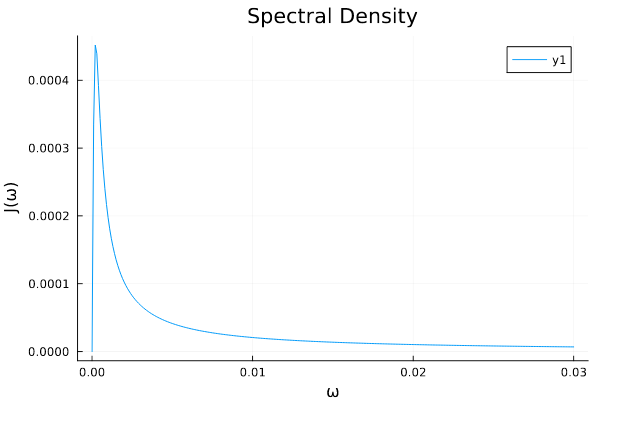
\includegraphics[scale=0.3]{Figures/jw_pentacene.png}
    \caption{Debye Spectral Density for Pentacene}
\end{figure}

Using calculations from the Quasi-Adiabatic Propagator Path Integral method, we can see the propagation of the density matrix. We can use this data to obtain the populations of the various sites (diagonal elements) and the coherences between the sites (off-diagonal elements).

\begin{figure}[h]
\centering
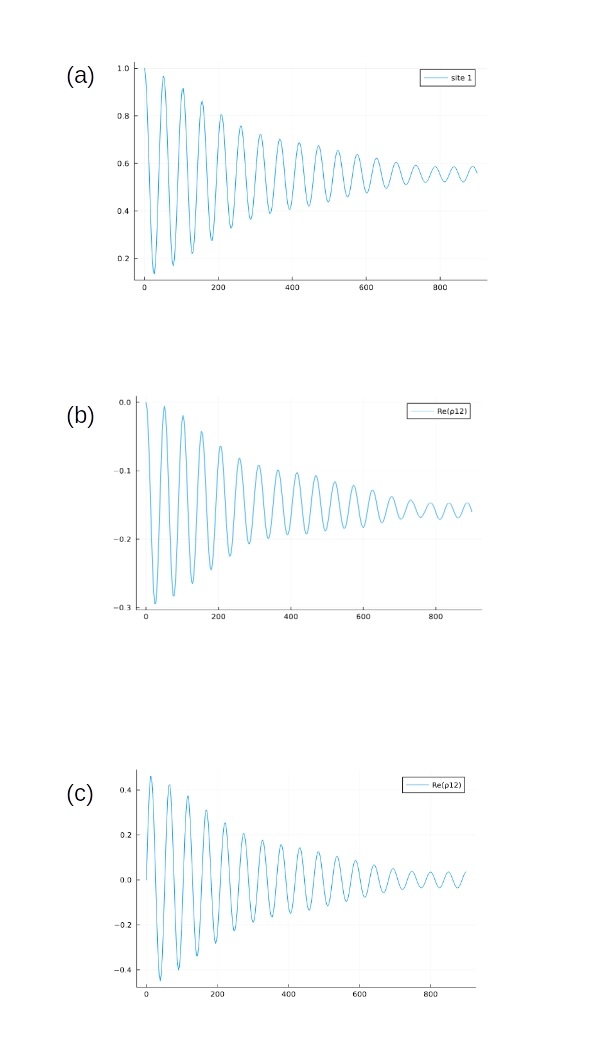
\includegraphics[scale=0.4]{Figures/pentacene_result}
\caption{Density Matrix Elements of Pentacene dimer. (a) $\rho_{11}$ population of site 1 (b) $Re(\rho_{12})$ Real part of coherence (c) $Im(\rho_{12})$ Imaginary part of coherence}
\end{figure}

%\begin{figure}
%\centering
%\includegraphics[scale=0.4]{Figures/pentacene_result2}
%\caption{Density Matrix Elements of Pentacene tetramer. (a) $\rho_{11}$ population of site 1 (b) $Re(\rho_{12})$ Real part of coherence (c) $Im(\rho_{12})$ Imaginary part of coherence}
%\end{figure}



\section{Rubrene}

Here, we attempt to model the dynamics of the Holstein-Peierls polaron in rubrene using the model developed by Ordejon, et al \cite{Ordejn2017}, where the Hamiltonian is given by :

\begin{equation}
    \mathcal{H} = \sum_{M,N} \epsilon_{MN} a_M^{\dag}a_N + \sum_{Q = (Z,P)} \omega_{Q} (b_Q^{\dag} b_{Q} + \frac{1}{2}) + \sum_{Q, M, N} \omega_{Q} g_{MN}^{Q}(b_{-Q} + b_{Q}^{\dag})a_M^{\dag}a_N 
\end{equation}

The effects of the bath are taken into consideration by the spectral density $J(\omega) = \sum_{i} g_i ^{2} \delta(\omega - \omega_i)$. We use a Gaussian line-shape broadening to model the spectral density $J(\omega)$.


\begin{figure}
    \center
    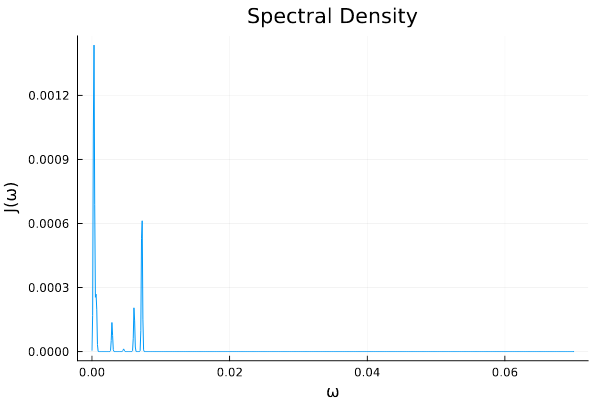
\includegraphics[scale=0.4]{Figures/jw_rubrene.png}
    \caption{Spectral Density (with Gaussian broadening) for Rubrene}
\end{figure}

We consider a simplified 1-dimensional chain of 10 rubrene sites with interactions between the nearest 2 neighbours.

By evaluating the QuAPI integral using tensor-train Monte carlo computations, we obtain the values of the RDM elements over time. We can use the diagonal elements to get the site populations.

\begin{figure}[h]
    \centering
    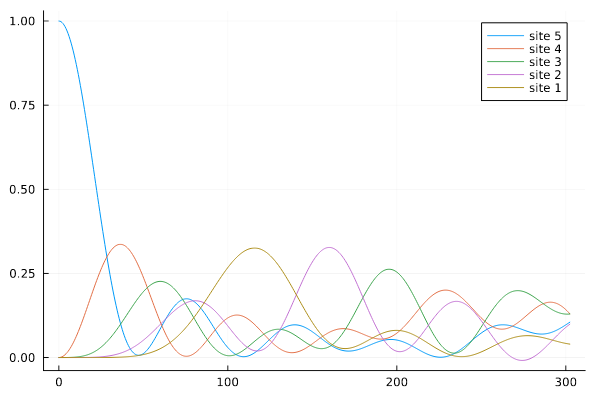
\includegraphics[scale=0.4]{Figures/rubrene_result.png}
    \caption{Populations of various sites in rubrene over time}
\end{figure}







%\input{Chapters/Chapter4}
%\input{Chapters/Chapter5}
%\input{Chapters/Chapter6}
%\input{Chapters/Chapter7}

%-------------------------------------------------------------------------------
%	THESIS CONTENT - APPENDICES
%-------------------------------------------------------------------------------

\addtocontents{toc}{\vspace{2em}} % Add a gap in the Contents, for aesthetics

\appendix % Cue to tell LaTeX that the following 'chapters' are Appendices

% Include the appendices of the thesis as separate files from the Appendices
% folder
% Uncomment the lines as you write the Appendices

% Appendix A

\chapter{Feynman Variational Approach to the Polaron Problem} % Main appendix title

\label{AppendixA} % For referencing this appendix elsewhere, use \ref{AppendixA}

\lhead{Appendix A. \emph{Feynman Variational Approach}} % This is for the header on each page - perhaps a shortened title



%% Appendix Template

\chapter{Spectral Line Broadening} % Main appendix title

\label{AppendixB} % Change X to a consecutive letter; for referencing this appendix elsewhere, use \ref{AppendixX}

\lhead{Appendix B. \emph{Spectral Line Broadening}} % Change X to a consecutive letter; this is for the header on each page - perhaps a shortened title


To approximate the line shape of a discrete spectrum when measured experimentally, we broaden the spectral lines using various methods.





%% Appendix Template

\chapter{Singular Value Decomposition} % Main appendix title

\label{AppendixC} % Change X to a consecutive letter; for referencing this appendix elsewhere, use \ref{AppendixX}

\lhead{Appendix C. \emph{Singular Value Decomposition}} % Change X to a consecutive letter; this is for the header on each page - perhaps a shortened title








\addtocontents{toc}{\vspace{2em}} % Add a gap in the Contents, for aesthetics

\backmatter

%-------------------------------------------------------------------------------
%	BIBLIOGRAPHY
%-------------------------------------------------------------------------------

\label{Bibliography}

\lhead{\emph{Bibliography}} % Change the page header to say "Bibliography"

\printbibliography

\end{document}
